\chapter{Débogage du Moteur KOOPT }
\label{chap:debogage du Moteur KOOPT }


Après la publication de la version beta de KOOPT pour donner la possibilité aux utilisateurs de tester l’application, on a pu cumuler les différents retours des testeurs,
qui concernent soit des bogues soit d'améliorations UX/UI (fonctionnalités,ergonomie)
  
Pour détecter les sources des différents problèmes, on a utilisé les LogCats pour nous aider à tracer l’exécution de l’émulateur et de l’application.
KOOPT dispose de ses propres Logs qui tracent l’exécution et le comportement de son moteur.
 
  \begin{figure}[H]
\begin{center}
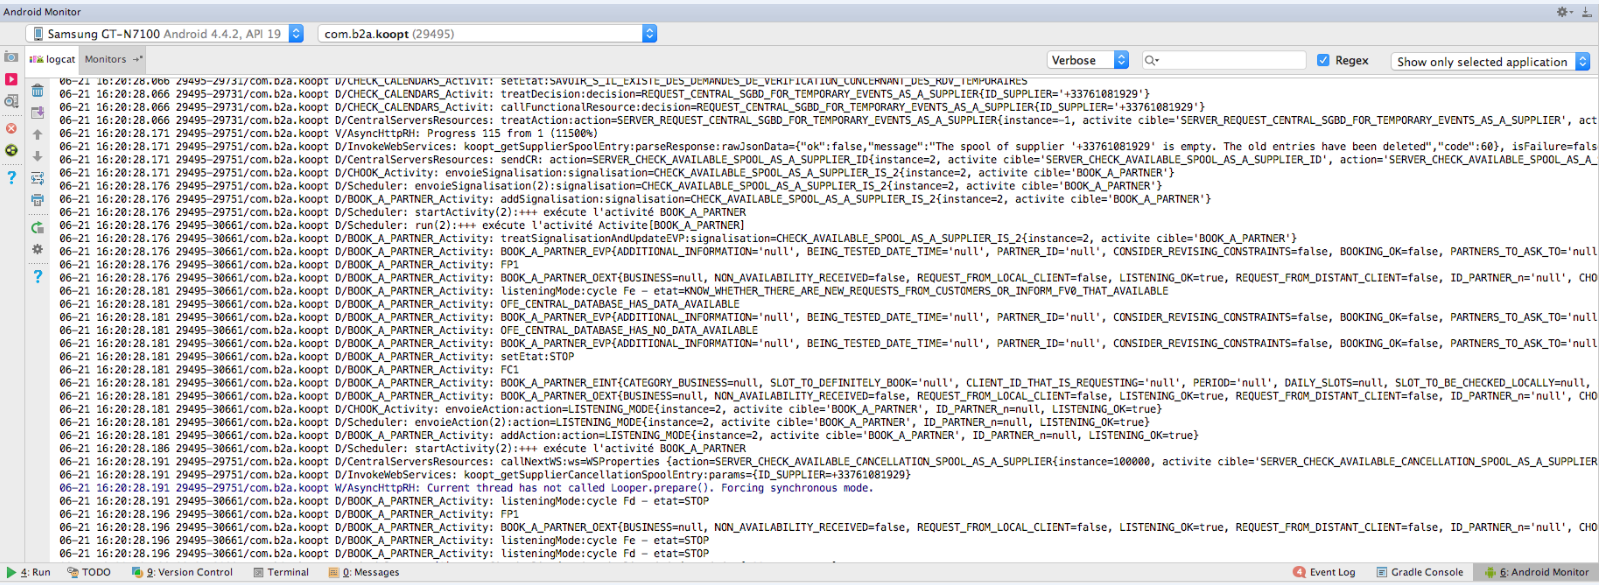
\includegraphics[width=1\linewidth]{images/androidmonitor}
\end{center}
\caption{Android Monitor}
\label{fig:19}
\end{figure}
 
Certains bugs proviennent de la conception de KOOPT, il était donc nécessaire d'interagir avec le responsable de la conception pour bien tracer le comportement du moteur et détecter la source de l’erreur.
 
